% Options here are passed to the article class.
% Most common options: 10pt, 11pt, 12pt
\documentclass[10pt]{datasheet}

% Input encoding and typographical rules for English language
\usepackage[utf8]{inputenc}
\usepackage[english]{babel}
\usepackage[english]{isodate}

% tikz is used to draw images in this example, but you can
% also use \includegraphics{}.
\usepackage{graphicx}

% These define global texts that are used in headers and titles.
\title{LC08: Precision Timings SIPO Register}
\author{Andrews54757}
\tags{logic-and-computation, register, sipo}
\date{21 December 2023}
\revision{Revision 1}
\begin{document}
\maketitle

\section{Features}

\begin{itemize}
\item{Expandable, QC based "stateless" logic}
\item{High precision timings support. Can discriminate order of signals sent in the same tick.}
\end{itemize}

\section{Applications}

\begin{itemize}
\item{Crackpot encoding mapping algorithm}
\end{itemize}

\section{General Description}
The LC08 Precision Timings Serial Input Parallel Output (SIPO) Register seperates input signals by order of input. The device is capable of discriminating between signals sent in the same tick. The device is expandable, and can be used to decode crackpot encoding schemes.

\vfill\break

\begin{figure}[h]
    \centering
    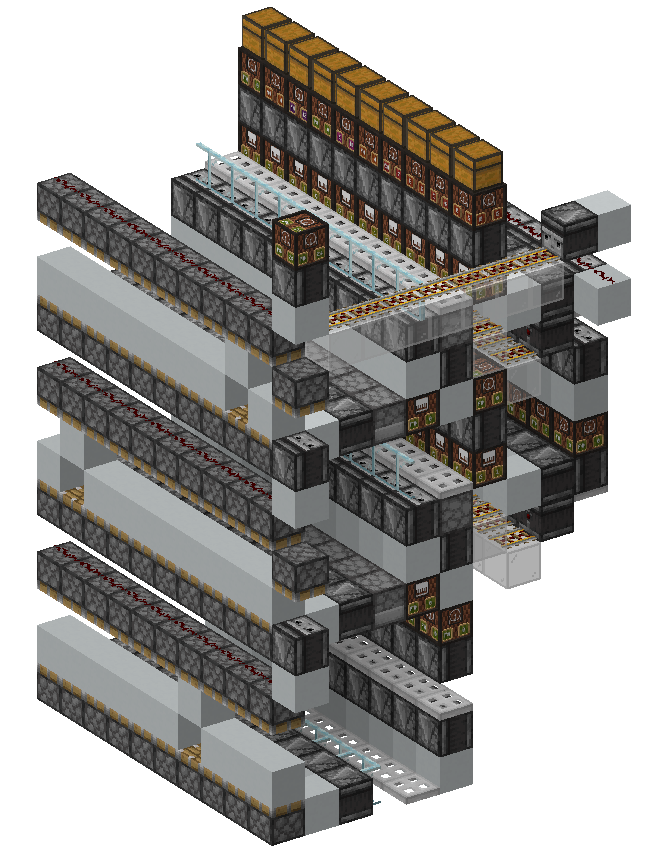
\includegraphics[width=0.48\textwidth]{sipo.png}
    \caption{\centering Precision Timings SIPO Register}
\end{figure}

% For wide tables, a single column layout is better. It can be switched
% page-by-page.
\onecolumn

\section{Device Specifications}

\begin{table}[h]
    \caption{Inputs}
    \begin{tabularx}{\textwidth}{l | c | X}
        \thickhline
        \textbf{Name} & \textbf{Range} & \textbf{Description} \\
        \hline
        Serial Input & Pulse & Noteblocks at the top \\
        \hline
        Reset & Pulse & Resets register \\
        \thickhline
\end{tabularx}
\end{table}

\begin{table}[h]
    \caption{Outputs}
    \begin{tabularx}{\textwidth}{l | c | X}
        \thickhline
        \textbf{Name} & \textbf{Range} & \textbf{Description} \\
        \hline
        Parallel Output & Pulse & Outputs at the bottom \\
        \thickhline
\end{tabularx}
\end{table}

\begin{table}[h]
    \caption{Device Specifications}
    \begin{tabularx}{\textwidth}{l | c c c | c | X}
        \thickhline
        \textbf{Parameter} & \textbf{Min.} & \textbf{Typ.} & \textbf{Max.} &
        \textbf{Unit} & \textbf{Conditions} \\
        \hline
        MC Version & 1.16 & 1.19.3 & - & MCV & Latest version at time of writing: 1.20.4\\
        \hline
        Dimensions & & 16 x 22 x 14 & & Blocks & \\
        \thickhline
\end{tabularx}
\end{table}
\newpage
\section{Testing Data}
\begin{table}[h]
\caption{Executed Tests}
\begin{tabularx}{\textwidth}{l | X}
    \thickhline
    \textbf{Test} & \textbf{Result} \\
    \hline
    SIPO test & Device was able to seperate signal order sent in same game tick. \\
    \thickhline
\end{tabularx}
\end{table}

\section{Download Information}
\begin{table}[h]
    \caption{Download Information}
    \begin{tabularx}{\textwidth}{l | l | l | X}
        \thickhline
        \textbf{Identifier} & \textbf{MC} & \textbf{File} & \textbf{Description} \\
        \hline
        LC08 & 1.19.3 & \href{https://github.com/Soontech-Annals/Archive/blob/8413f90a054b6c415703bae02badeba7541344f6/Archive/logic-and-computation/LC08\%20Precision\%20Timings\%20SIPO\%20Register/LC08\_Precision\_Timings\_SIPO\_Register.litematic?raw=1}{LC08\_Precision\_Timings\_SIPO\_Register.litematic} & Schematic of device. \\
        \hline
        \thickhline
    \end{tabularx}
\end{table}

\end{document}

